\section{Bootstrap}
%https://www.internet-exposure.com/blog/standalone-mobile-websites-vs-responsive-design/
Immer mehr Smartphones, Tablets und andere Mobilgeräte werden genutzt, um im Internet zu surfen. Weltweit werden 68 Millionen Google-Suchanfragen pro Stunde auf Mobilgeräten durchgeführt. Laut StatCounter waren im Juli 2018 52,95\% des weltweiten Internetverkehrs auf einem Mobilgerät. Weitere 3,94\% kamen von Tablets \cite{statCounter}. Das bedeutet, dass Mobile Nutzer einen großen Einfluss haben, mit dem man rechnen muss um den langfristigen Erfolg sicherzustellen. Es gibt zwei Optionen zum Erstellen einer für Mobilgeräte optimierten Website. Man kann eine separate mobile Website oder eine Responsive-Website entwickeln.
 
\subsection{Eigenständige mobile Website (Separate mobile Website)}
%Mobile-dedizierte Websites
Separate mobile Websites sind Websites, die speziell für Mobilgeräte entwickelt wurden. Sie leben häufig unter einer separaten URL (z.B. \textit{m.site.de}) und unterscheiden sich von der vollständigen Website. Sie enthalten Funktionen oder Inhalte, die für Mobilgeräte als geeignet erachtet wurden. Häufig sind dies nur einige der auf dem Desktop verfügbaren Komponenten. 
%(muss noch umschreiben)Sie stehen oft im Gegensatz zu Responsive-Websites, die für Mobilgeräte und Desktops in der Regel dieselben Inhalte und Funktionen enthalten, diese jedoch auf Mobilgeräten neu anordnen. 
Eine separate mobile Website bietet Differenzierung von mobilen Inhalten und erstellt ein vollständig mobiles Benutzererlebnis.

%http://todayslocalmedia.com/standalone-mobile-site-vs-mobile-responsive-site/
Das größte Problem mit separaten mobilen Websites besteht darin, dass man zwei separate Websites erstellen und verwalten muss. Wenn man Änderungen an der einen Website vornehmen muss, muss man dieselben Änderungen auf der anderen Website wiederholen. Dies könnte mehr Zeit und Geld kosten. Auch wenn man es auf einer separaten Domain platziert, muss man für eine neue Domain und das Hosting bezahlen. Die Umleitung kann die Ladezeit beeinflussen, was die Absprungrate erhöhen kann, da Besucher ungeduldig sein können.

% Aber der große Nachteil der Erstellung einer separaten Website besteht darin, dass viel mehr Wartung erforderlich ist, um die zwei Versionen (eine für Mobilgeräte und eine für Desktop) einer Website homogen zu halten.

\subsection{Sich anpassendes Design (Responsive-Design)}
Der Begriff Responsive-Design, zuerst von Ethan Marcote im Jahr 2010 geprägt, beschreibt eine Entwicklungstechnik, bei der das Design einer Website automatisch an die Größe der Benutzerbildschirme angepasst wird. Daher kann derselbe Inhalt in einem dreispaltigen Format auf einem Desktop, einem zweispaltigen Format auf einem Tablet und einem einspaltigen Format auf einem Smartphone angezeigt werden. Kurztipp: Man kann feststellen, ob eine Website ``responsive'' ist, indem man das Browserfenster manuell vergrößert oder verkleinert.

Responsive-Design liefert für jede Seite unabhängig vom Gerät den gleichen Code über eine einzige URL an den Browser. Man muss nicht mehr zwei Versionen einer Website erstellen: eine für Desktop-Computer und eine für mobile Geräte. Da es sich nur um eine Website handelt, ist eine Responsive-Website einfacher und kostengünstiger zu warten. Alle Änderungen, die man vornimmt, sind sowohl in der mobilen Version als auch in der Desktop Version sichtbar. Außerdem sind Responsive-Websites oft einfacher zu implementieren und weniger kompliziert in Bezug auf die Konfiguration für Suchmaschinen.

%https://alphadigital.com.au/blog/responsive-adaptive-dedicated-mobile-sites/
Es gibt jedoch auch Nachteile, die mit Responsive-Design einhergehen. Da eine Responsive-Website als eine einzelne Entität codiert ist (im Gegensatz zu einer Desktop-Website und dann einer separaten mobilen Website), müssen alle Seitenressourcen und Code für jeden Besuch des Benutzers heruntergeladen werden, unabhängig von der Bildschirmgröße oder Gerät, das sie besuchen. In mobilen Versionen von Responsive-Website werden häufig bestimmte Elemente nicht angezeigt, um Webseiten oder Abschnitte benutzerfreundlicher zu machen. Diese Elemente müssen jedoch ``unsichtbar'' geladen werden. Dies bedeutet, dass die Webseiten mit dem Responsive-Design wahrscheinlich langsamer geladen werden.

%Sodass ist das Responsive-Design wartungsfreundlich, 
%Dagegen hat Responsive-Design auch einige Nachteile wie bei große Seiten, die für den Desktop geeignet sind, werden möglicherweise nur langsam auf Mobilgeräte geladen. Außerdem könne die Elemente können sich bewegen, daher bietet Responsive-Design keine vollständig mobile Benutzererfahrung.

%Der grafische Aufbau einer Responsive-Website erfolgt anhand der Anforderungen des jeweiligen Gerätes, mit dem die Website betrachtet wird. Dies betrifft insbesondere die Anordnung und Darstellung einzelner Elemente, wie Navigationen, Seitenspalten und Texte, aber auch die Nutzung unterschiedlicher Eingabemethoden von Maus (klicken, überfahren) oder Touchscreen (tippen, wischen). Technische Basis hierfür sind die neueren Webstandards HTML5, CSS3 (hier insbesondere die Media Queries) und JavaScript\footnote{\url{https://de.wikipedia.org/wiki/Responsive_Webdesign}}.




%Vorteil
%\begin{itemize}
%\item	Leichter und kostengünstiger zu warten.
%\item	Eine URL für alle Geräte. Keine Notwendigkeit für komplizierte Annotation.
%\item	Keine komplizierte Erkennung und Umleitung von Geräten erforderlich.
%\item	Uniform & nahtlose = gute UX.
%\item	Fülle der zu verwendenden Vorlagen.
%\item	SEO freundlich.
%\item	Oft einfacher zu implementieren
%\end{itemize}

%Nachteil
%\begin{itemize}
%\item	Große Seiten, die für den Desktop geeignet sind, werden möglicherweise nur langsam auf Mobilgeräte geladen.
%\item	Bietet keine vollständig mobile Benutzererfahrung.
%\item	Weniger Bildschirmgröße Design-Steuerelement.
%\item	Elemente können sich bewegen
%\item	Anzeigen auf dem Bildschirm verloren.
%\item	Längere mobile Downloadzeiten
%\end{itemize}

\subsection{Mobile-first}
Außerdem gibt es noch die Begriffe ``Desktop-First'' und ``Mobile-First''. Während Responsive-Design eine Entwicklungstechnik ist, sind Desktop-First und Mobile-First die Design-Strategien\cite{Gonzalo}.

Desktop-First ist ein Konzept im Responsive-Design bei dem als erstes die Website für die Desktop-Darstellung entwickelt wird. Für kleinere Displays wird die Seite im Nachhinein angepasst\cite{kulturbanause}.\\
Mobile-First, eine Idee von Luke Wroblewski, ist ein Trend in der Website-Entwicklung, bei der das Entwerfen einer Website für Smartphones, Tablets und mobilen Geräte Vorrang vor der Desktop-Version hat. Mit Mobile-First wird ein Webdesigner angesichts der Einschränkungen einer mobilen Plattform (kleiner Bildschirm, langsamere Prozessoren) eine Website erstellen und dann die Website entweder für die Desktop Nutzung kopieren oder verbessern.

\begin{figure}[ !h] \centering
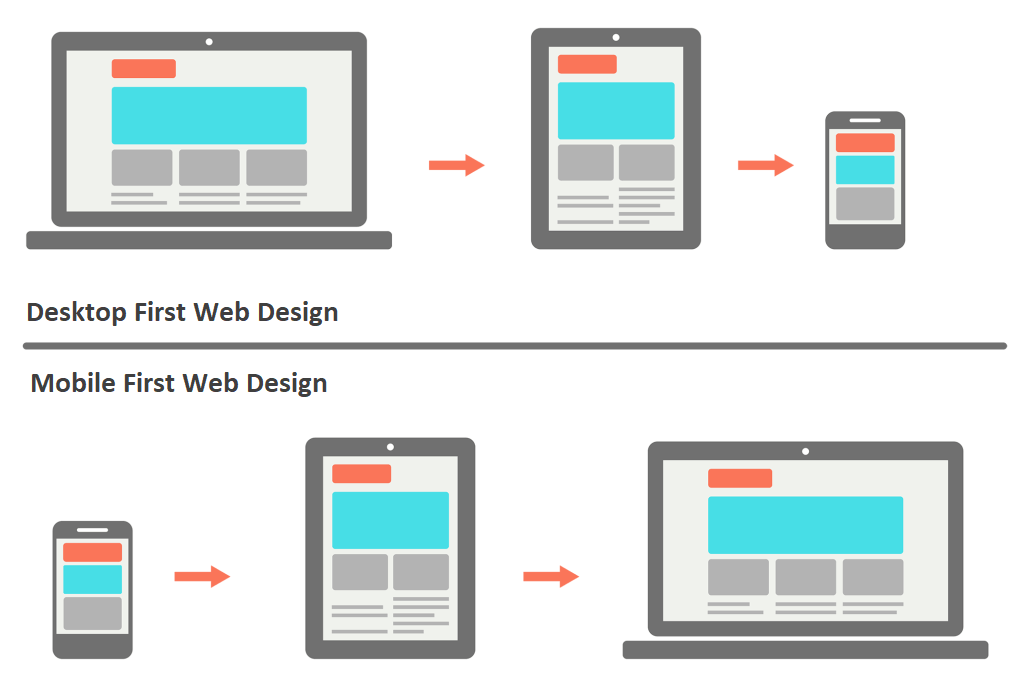
\includegraphics[width=1.0\textwidth]{DesktopMobileFirst}
\caption[Desktop-First und Mobile-First]{Desktop-First und Mobile-First\\ Quelle: \url{http://fredericgonzalo.com/en/2017/03/01/understanding-the-difference-between-mobile-first-adaptive-and-responsive-design/}}\label{fig:DesktopMobileFirst}
\end{figure}

\subsection{Bootstrap} \label{Bootstrap}
Aufgrund der Unterstützung für die Informatik Studierenden (\hyperlink{/LE10/}{/LE10/}und \hyperlink{/LE40/}{/LE40/}), die den Laptop fast täglich verwenden müssen, den Wartungsaufwand und die Implementierungskomplexität, wird eine Responsive-Website mit ``Laptop-First'' Strategie (Bildschirmgröße $\geq$ 768 px) gewählt. Um eine Responsive-Website schneller und einfacher gestalten zu können, wird Bootstrap verwendet.

Bootstrap ist ein beliebtes, kostenloses HTML-, CSS- und JavaScript-Framework zum Entwickeln von Responsive-Websites mit Priorisierung von Mobilgeräten. Das Framework enthält Responsive-CSS- und -HTML-Vorlagen für Schaltflächen, Tabellen, Navigation, Bildkarussells und andere Elemente, die man auf der Webseite verwenden kann. Es sind einige optionale JavaScript-Plugins verfügbar, die selbst Entwicklern mit lediglich grundlegenden Codierungskenntnissen das Entwickeln großartiger Responsive-Websites ermöglichen. Bootstrap ist mit allen modernen Browsern kompatibel wie (\hyperlink{/LE10/}{Chrome}), Firefox, Internet Explorer, Safari und Opera \cite{bootstrapworld}.

\begin{figure}[ !h] \centering
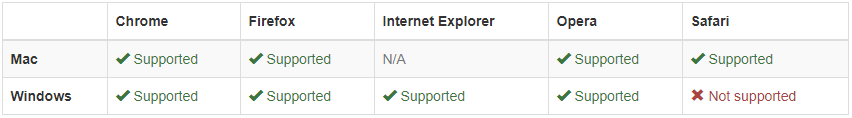
\includegraphics[width=1.0\textwidth]{DesktopBrowsers}
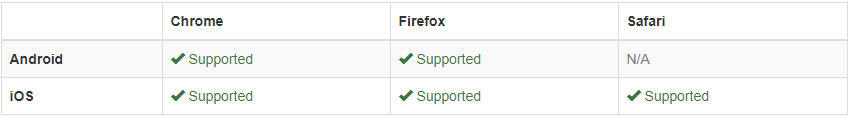
\includegraphics[width=1.0\textwidth]{MobileBrowsers}
\caption[Unterstützte Browsers von Bootstrap]{Unterstützte Browsers von Bootstrap\\ Quelle: \url{https://getbootstrap.com/docs/3.3/getting-started/\# support}}\label{fig:DesktopMobileBrowsers}
\end{figure}

Bootstrap wurde 2010 von Twitter unter dem Namen „Twitter Bootstrap“ entwickelt, mit dem Ziel eine einheitliche Bibliothek für die Gestaltung von Weboberflächen zu schaffen. Das Problem war damals, dass für die Designentwicklung bei Twitter viele verschiedene Bibliotheken verwendet wurden. Das führte zu Inkonsistenzen und einem großen Wartungsaufwand. Bootstrap sollte eine gemeinsame Basis schaffen, mit der alle Mitarbeiter arbeiten konnten, um schnell und einfach Websites zu gestalten.
Im August 2011 entschloss sich Twitter dazu, das Bootstrap Framework als Open Source Projekt zu veröffentlichen. Damit war der Siegeszug dieses ausgezeichneten und leicht zu bedienenden Frontend-Frameworks zur Webdesign-Gestaltung nicht mehr aufzuhalten\cite{bootstrap}.

Um Bootstrap zu verwenden, muss man HTML und CSS nicht gut kennen. Es ist ein Vorteil, wenn man ein Backend-Entwickler ist und einige UI-Änderungen vornehmen kann. 
%Bootstrap ist vollständig anpassbar, man kann wählen, welche Komponenten man verwenden möchte und verwendet eine Variablen-Datei, um noch mehr Farbe und Verhalten zum Anpassung zu bekommen. Alles, was man tun muss, ist es die Seite \url{http://getbootstrap.com/customize/} zu besuchen. Dann wählt man die benötigten Plugins aus und klickt man auf Downloaden. 
%Bootstrap bietet auch eine Möglichkeit, die internen Variablen für fortgeschrittene Benutzer zu überschreiben, aber sie bieten ziemlich ordentliche Standardwerte, so dass man sich darüber keine Gedanken machen sollte, es sei denn, man muss dies tun.

%Bootstrap bietet viele Hilfsklassen, die die Entwicklung einer responsiven Website einfach und schnell machen. Man kann jedes Layout mit fester Breite in ein flüssiges Layout umwandeln, indem man einfach seine übergeordnete \textit{.container} Klasse in \textit{.container-fluid} ändern. Bootstrap verfügt außerdem über die Klassen \textit{.visible}, mit denen man steuern kann, wie seine Section auf Tablets und mobilen Geräten angezeigt werden. Beispiel:
%
%\textit{<div class = ``sichtbarer-xs-block visible-sm-block''> </ div>}
%
%In diesem Fall wird das div als ein Section mit display angezeigt: block nur auf Telefonen und Tablets. Es wird auf dem Desktop versteckt werden.

%Um Bootstrap in einer HTML-Seite zu verwenden, muss lediglich ein fertiges ZIP-Archiv von der Bootstrap-Webseite \url{http://getbootstrap.com/docs/3.3/getting-started/\# download} heruntergeladen werden. 
Bootstrap-Bibliothek kann als ein ZIP-Archiv von der Bootstrap-Webseite \url{http://getbootstrap.com/docs/3.3/getting-started/\# download} heruntergeladen werden. Dieses Archiv enthält bereits fast alle benötigten, in das eigene Projekt einzubindenden Dateien, wie eine Stylesheetdatei mit allen Komponenten, eine JavaScript-Datei mit allen Plugins und auch eine benötigte Icon-Schriftart. Alternativ gibt es auf GitHub noch ein vollständiges, deutlich umfangreicheres ZIP-Archiv für Entwickler herunterzuladen, welches auch Beispiele für typische Webseiten zur bequemen Verwendung als Ausgangsdatei und vieles weitere enthält.

Die Dateien im ZIP-Archiv müssen in das eigene HTML-Dokument/Projekt eingebunden werden. Soll auch mit JavaScript-Komponenten gearbeitet werden, so muss die JavaScript-Datei zusammen mit der jQuery-Bibliothek ebenfalls im HTML-Dokument referenziert werden. Möchte man angepasste Einstellungen für Stil und JavaScript-Funktionalität, besteht die Möglichkeit, fast alle Elemente von Bootstrap auf der Website selbst zu verändern und ein angepasstes Paket herunterzuladen. Schließlich kann man Bootstrap auch lokal, seinen Bedürfnissen entsprechend, vom Standard abweichend kompilieren.

Das folgende Beispiel verdeutlicht die Funktionsweise. Der HTML-Quellcode definiert ein einfaches Suchformular sowie eine Ergebnisliste in Form einer Tabelle. Die Seite besteht aus regulären, semantisch verwendeten HTML5-Elementen sowie einigen zusätzlichen CSS-Klassenangaben entsprechend der Bootstrap-Dokumentation \cite{bootstrapwiki}.

\lstinputlisting[language=HTML, caption=Bootstrap Beispiel, basicstyle=\scriptsize]{ex.html}
%\begin{lstlisting}[language=HTML, caption=Bootstrap Beispiel]
%<!DOCTYPE html>
%<html>
%
%  <head>
%    <title>Bootstrap Beispiel</title>
%
%    <!-- Einbinden des Bootstrap-Stylesheets -->
%    <link rel="stylesheet" href="https://ajax.aspnetcdn.com/ajax/bootstrap/3.3.7/css/bootstrap.min.css">
%
%    <!-- optional: Einbinden der jQuery-Bibliothek -->
%    <script src="https://ajax.aspnetcdn.com/ajax/jQuery/jquery-1.12.4.min.js"></script>
%
%    <!-- optional: Einbinden der Bootstrap-JavaScript-Plugins -->
%    <script src="https://ajax.aspnetcdn.com/ajax/bootstrap/3.3.7/bootstrap.min.js"></script>
%  </head>
%
%  <body>
%    <section class="container">
%      <h1>Suche</h1>
%      <p>Beispiel für ein einfaches Suchformular.</p>
%      <!-- Suchformular mit Eingabefeld und Button -->
%      <form class="well form-search">
%        <input type="text" class="input-medium search-query"/>
%        <button type="submit" class="btn btn-primary">Search</button>
%      </form>
%
%      <h2>Ergebnisse</h2>
%      <!-- Tabelle mit abwechselnder Zellenhintergrundfarbe und Ausserrahmen -->
%      <table class="table table-striped table-bordered">
%     
%      </table>
%    </section>
%  </body>
%
%</html>
%\end{lstlisting}

\textbf{Grid System}

Das Grid-System ist eines der wichtigsten Konzepte in Bootstrap, das beschreibt, wie man Komponenten auf der Oberfläche positionieren und wie man eine Responsive-Website implementieren kann. Im Grid-System ist das Layout der Seite in verschiedene Zeilen aufgeteilt. Jede Zeile hat maximal 12 Spalten (möglicherweise weniger). Basierend auf der Breite des Anzeigegerätetyps kann man verschiedene CSS-Klassen verwenden, um die Anzahl der Anzeigespalten anzupassen. Zum Beispiel hat man eine Webseite, die das Grid Layout System wie folgt verwendet:  

\begin{figure}[ !h] \centering
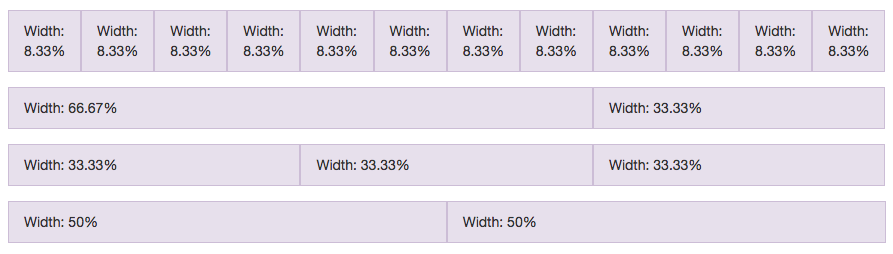
\includegraphics[width=1.0\textwidth]{BootstrapGridSystem}
\caption[Beispiel Grid System]{Beispiel Grid System}\label{fig:BootstrapGridSystem}
\end{figure}

Die Abbildung \ref{fig:BootstrapGridSystem} hat vier verschiedene Zeilen, wobei jede Zeile eine andere Anzahl von Spalten hat, beispielsweise die erste Zeile hat 12 Spalten. Die CSS-Klasse, die auf die Spalte angewendet wird, ist in fünf verschiedene Kategorien unterteilt (Tabelle \ref{tab:BootstrapGridSystem}). 

\begin{table}[h]
\footnotesize
	\begin{center}
			\begin{tabular}{|l|c|c|c|c|c|}
			\hline
			&\textbf{Extra klein}&\textbf{Klein}&\textbf{Medium}&\textbf{Groß}&\textbf{Extragroß}\\
			& <576px & $\geq$ 576px & $\geq$ 768px&$\geq$ 992px &$\geq$ 1200px\\
			\hline
			\textbf{Maximale }&Keine&540px&120px&960px&1140px\\
			\textbf{Behäterbreite}&(automatisch)&&&&\\
			\hline
			\textbf{Klassenpräfix}&.col-&.col-sm-&.col-md-&.col-lg-&.col-xl-\\
			\hline
			\textbf{Anzahl der Spalten}&\multicolumn{5}{|c|}{12}\\
			\hline
			\textbf{Stegbreite}&\multicolumn{5}{|c|}{30px(15px auf jeder Seite einer Spalte)}\\
			\hline
			\textbf{Nestbar}&\multicolumn{5}{|c|}{Ja}\\
			\hline
			\textbf{Spaltenbestellung}&\multicolumn{5}{|c|}{Ja}\\
			\hline
			\end{tabular}
	\end{center}
	\caption[Rasteroptionen im Bootstrap-Framework]{Rasteroptionen\\Quelle: https://getbootstrap.com/docs/4.1/layout/grid/}
	\label{tab:BootstrapGridSystem}
\end{table}		

Wenn es nur 1 Block \textit{<div class=``col-md''> </div>} und keine Spaltennummer gibt, ist der Standardwert 12 Spalten (voller Block von Containern). Wenn man 3 Blöcke \textit{<div class=``col-md''> </div>} hat, werden die Blöcke automatisch ebenso wie \textit{<div class=``col-md-4''> </div>} unterteilt. Die Bildschirme, die größer als den verwendeten Bildschirm sind, ändern sich nicht. Die kleineren Bildschirme werden automatisch auf \textit{col-12} (eine Spalte pro Zeile) umgeschaltet, wenn keine andere Anpassung vorgenommen wird. Das folgende Beispiel verdeutlicht die Funktionsweise des Grid System.

Zuerst fügt man dieses Meta-Tag dem Head-Tag hinzu.
\begin{lstlisting}[language=HTML, basicstyle=\scriptsize]
<meta name="viewport" content="width=device-width, initial-scale=1.0">
\end{lstlisting}	
Und das Body-Tag ist wie folgt:
\begin{lstlisting}[language=HTML, caption= Beispiel Grid System,basicstyle=\scriptsize]
<div class="container" style="background-color: grey; margin-bottom: 50px;">
   <div class="row">
      <div class="col-md-4 col-sm-6">
         <div class="block"></div>
      </div>
      <div class="col-md-8 col-sm-6">
         <div class="block"></div>
      </div>
   </div>
</div>
\end{lstlisting}
Ergebnisse des Laufs des obigen Codes:
\begin{itemize}
\item Wenn die Bildschirmbreite größer als 768px ist, wird jede Zeile in zwei Spalten aufgeteilt: Eine Spalte belegt 33,33 \% der Bildschirmbreite und eine Spalte belegt 66,67 \% der Bildschirmbreite.
\item  Wenn die Bildschirmbreite weniger als 768px ist, wird jede Zeile in zwei Spalten aufgeteilt: Jede Spalte belegt 50\% der Bildschirmbreite.
\item Wenn die Bildschirmbreite weniger als 576px ist, hat jede Zeile nur eine Spalte.
\end{itemize}

Die Dokumentation von Bootstrap ist essentiell. Bootstrap hat eine umfangreiche Dokumentation inklusive Demos, die auch für Anfänger in dem Bereich leicht nachvollziehbar sind und bis hin zu den komplexesten Elementen alles für den Nutzer zugänglich macht. Unter \url{http://getbootstrap.com/getting-started/\# template} kann man eine grundlegende Vorlage und eine Reihe von Beispielen für unterschiedliche Bedürfnisse \url{http://getbootstrap.com/getting-started/\# examples} herunterladen. Man kann einfach das Bootstrap-Repository herunterladen, in den Ordner \textit{docs / examples} gehen, das gewünschte Beispiel kopieren / einfügen und daran arbeiten.
%https://www.htmlgoodies.com/html5/markup/10-common-uses-of-bootstrap.html


%1. Zunächst ist Bootstrap das beliebteste Framework zum Erstellen von Layouts. Hier sind einige zusätzliche Gründe Bootstrap zu verwenden:
%
%Das reaktionsschnelle CSS von Bootstrap passt sich an Telefone, Tablets und Desktops an
%Mobile-First-Styles sind Teil des Frameworks
%Bootstrap ist mit allen modernen Browsern kompatibel (Chrome, Firefox, Internet Explorer, Safari und Opera).
%2. Bootstrap hat eine große Community und freundlichen Support. Für Ressourcen besuchen Sie:
%Schau dir den Bootstrap Blog an.
%Sie können mit Bootstrappern mit IRC im irc.freenode.net Server im ## bootstrap channel chatten.
%Schaut euch an, was die Leute mit Bootstrap auf der Bootstrap Expo machen.
%3. Bootstrap ist einfach einzurichten und ein funktionierendes Layout in weniger als einer Stunde zu erstellen
%
%Sie haben eine grundlegende Vorlage unter http://getbootstrap.com/getting-started/#template und eine Reihe von Beispielen für unterschiedliche Bedürfnisse (http://getbootstrap.com/getting-started/#examples). Sie können einfach das Bootstrap-Repository herunterladen, in den Ordner docs / examples gehen, das gewünschte Beispiel kopieren / einfügen und daran arbeiten.
%
%4. Sie müssen HTML und CSS nicht gut kennen, um Bootstrap zu verwenden, es ist ein Vorteil, wenn Sie ein Backend-Entwickler sind und einige UI-Änderungen vornehmen müssen.
%
%5. Es ist vollständig anpassbar, ich kann wählen, welche Komponenten ich verwenden möchte und verwenden Sie Variablen-Datei, um noch mehr Farbe und Verhalten Anpassung zu bekommen.
%
%Alles, was Sie tun müssen, ist http://getbootstrap.com/customize/, wählen Sie die benötigten Plugins aus und klicken Sie auf Download. Bootstrap bietet auch eine Möglichkeit, die internen Variablen für fortgeschrittene Benutzer zu überschreiben, aber sie bieten ziemlich ordentliche Standardwerte, so dass Sie sich darüber keine Gedanken machen sollten, es sei denn, Sie müssen dies tun.
%
%6. Wenn Sie die Bootstrap-Version aktualisieren, werden Sie nicht viele Fehler sehen, da sich das Kernteam um die Abwärtskompatibilität kümmert.
%
%7. Ihre Dokumentation ist großartig! Hier sind einige Ressourcen zum Auschecken:
%
%Bootstrap 3 Tutorial
%Code Academy: Bootstrap
%Webdesign-Tutorials: Bootstrap
%8. Bootstrap bietet viele Hilfsklassen, die die Entwicklung einer responsiven Website einfach und schnell machen.
%
%Sie können jedes Layout mit fester Breite in ein flüssiges Layout umwandeln, indem Sie einfach Ihre übergeordnete .container-Klasse in .container-fluid ändern.
%
%Bootstrap verfügt außerdem über die Klassen .visible - * - *, mit denen Sie steuern können, wie Ihre Abschnitte auf Tablets und mobilen Geräten angezeigt werden. Beispiel:
%
%<div class = "sichtbarer-xs-block visible-sm-block"> </ div>
%
%In diesem Fall wird das div als ein Abschnitt mit display angezeigt: block nur auf Telefonen und Tablets. Es wird auf dem Desktop versteckt werden.
%
%9. Bootstrap-Komponenten sind gut in das Ökosystem der beliebten JS MVC Frameworks wie Angular übernommen. Bootstrap bietet mehrere Möglichkeiten, es in Ihr Projekt einzubinden:
%
%Benutzung der Laube:
%
%Bower installieren Bootstrap
%
%Verwenden von npm:
%
%npm install bootstrap
%
%Und einfach ein Skript-Tag mit der URL hinzufügen, um Source auf CDN zu laden.
%
%Wir haben auch ui-bootstrap für Angular.js und react-bootstrap für React. Sie können sie auch über Bower und Npm installieren. Um zum Beispiel ein Kollaps-Element zu erstellen, müssen Sie nur ein ähnliches Markup erstellen:
%
%<div uib-collapse = "isCollapsed">
%
%<div class = "well well-lg">
%
%Inhalt des Einsturzes
%
%</ div>
%
%</ div>
%
%Anstatt eine Menge jQuery-Konfiguration zu machen, wie Sie es normalerweise tun würden.
%
%10. Bootstrap löst viele browserübergreifende Probleme auf und Sie müssen sich nicht ständig darum kümmern.
%
%Hinweis: Bootstrap wurde für die Verwendung mit den neuesten Desktop- und mobilen Browsern entwickelt. Dies bedeutet, dass die Anzeigen in älteren Browsern möglicherweise anders aussehen und möglicherweise anders gerendert werden, obwohl die Anzeigen gemäß der Dokumentation voll funktionsfähig sein sollten.
%
%Hier sind ein paar Screenshots zur Browserkompatibilität.







%Note
%https://www.nngroup.com/articles/mobile-vs-responsive/
%\url{https://www.clickseed.com/responsive-design-vs-separate-mobile-site-vs-dynamic-serving/}
%\url{https://www.interaction-design.org/literature/article/adaptive-vs-responsive-design}